\chapter{Experimental setup}
\label{ch:exp}

\intro{The measurements within this thesis are based on \acrfull{pp} collision data recorded with the \gls{cms} detector in 2012, 2015, and 2016 at \acrlong{cm} energies of 8 and 13~TeV. In this chapter the experimental setup is described. First, an overview of the \gls{lhc}, its preacceleator chain and the experiments at the \gls{lhc} is given. Then, the \gls{cms} detector and its major components are detailed which are: the solenoid magnet, the inner tracking system, the electromagnetic and hadronic calorimeters, and the muon system. The chapter is concluded with a brief introduction to the trigger and data acquisition system of the \gls{cms} experiment.}

%##############################################
\section{Large Hadron Collider}
%##############################################

The \glshere{lhc} is a 26.7~km long accelerator and storage ring for protons and heavy ions located at the \glshere{cern} in the vicinity of Geneva, Switzerland~\cite{Evans:2008zzb}. It was constructed between 1998\range2008 in the existing tunnel of the former \glshere{lep} which lies 45\range170~m below the surface of Switzerland and France. The \gls{lhc} ring features two beam pipes which can be separately filled with up to 2\,808 countercycling bunches per pipe with a bunch spacing of 25~ns. The two beams can be focused to cross each other at four \glsplhere{ip}. The design allows to accelerate protons with a momentum of 450~\GeV at injection to up to 7~\TeV yielding a maximum \acrlong{cm} energy of 14~\TeV in collisions.

The beams are bent by 1\,232 dipole cryostats that host both beam pipes and corresponding dipole magnets within a cold mass in a twin-bore design. The cold mass itself is placed in a vacuum vessel for thermal insulation. The magnet coils consist of \glshere{nbti}  cables which are cooled down to 1.9~K using superfluid helium. At this temperature, the \gls{nbti} alloy is superconducting. This allows to produce the required dipole field strength ranging from 0.54~T at injection to up to 8.33~T at the maximum beam energy for sustaining a closed beam orbit. Such high magnetic fields cannot be achieved with normal conductors due to magnetic saturation which is why the coils have to be superconducting. At maximum field a current of 11850~A is required. In addition to the dipole magnets about 3\,800 single aperture and 1\,000 twin aperture magnets are installed. Quadrupole magnets keep the beam particles focused around the nominal orbit. Further, non-linear corrections to the orbit are applied using sextu-, octu-, and decapoles. Special quadrupole triplets at each side of the four \glspl{ip} focus the beams for collision. The envelope of the particle trajectories with respect to the nominal beam orbit is described by the betatron function which can be approximated around the \glspl{ip} as 

\begin{equation}
\beta(x)\approx\beta^\star+\frac{x^2}{\beta^\star}\,,
\end{equation}

where $x$ denotes the distance to the focal point. In design the beams can be squeezed to $\beta^\star=0.55~\mathrm{m}$ at two high luminosity \glspl{ip}. The transverse beam size at the \glspl{ip} can be calculated as $r=\sqrt{\epsilon_\mathrm{n}\cdot\beta^\star/\gamma}\approx17\upmu\mathrm{m}$ for $\gamma=E_\mathrm{p}/m_\mathrm{p}=7\,000$, where $\epsilon_\mathrm{n}$ denotes the normalized beam emittance. The emittance is a measure of the phase space area occupied by the particles within the beam which is constant in a closed system following Liouville's theorem. For the \gls{lhc} it cannot be larger than $\epsilon_\mathrm{n}>3.75~\upmu\mathrm{m}\cdot\mathrm{rad}$ in order not to loose significant amounts of the beam intensity in the \gls{lhc} arcs where $\beta(x)$ is the largest.

For acceleration and longitudinal focusing of the bunches, a system of eight superconducting cavities per beam with a resonance frequency of $400.8~\mathrm{MHz}$ are installed. This matches the 35\,640~harmonic mode of the beam revolution frequency of $f_\mathrm{rev}=11\,245~\mathrm{Hz}$. The cavity system yields an energy gain per turn of 485~keV which results in an acceleration time of about 20~min from injection to the maximum beam energy.

The expected luminosity at the \glspl{ip} can be calculated from the introduced machine and beam parameters as

\begin{equation}
L=\frac{N_\mathrm{p}^{2}\,n_\mathrm{b}\,f_\mathrm{rev}}{4\pi\,d^2_{x,y}}\cdot F,\qquad F=\frac{1}{\sqrt{1+\big(\theta\cdot d_{z}\big)^2\big/\big({2\,d_{x,y}}\big)^2}}\,,
\end{equation}

where $N_\mathrm{p}$ denotes the number of protons per bunch and $n_\mathrm{b}$ the number of colliding bunches. The design proton population per bunch is $N_\mathrm{p}=1.15\cdot10^{11}$. The factor $F$ accounts for a reduction in luminosity due to a slight tilting of the beams by the crossing angle $\theta$. In 2016, the design luminosity of $10^{34}~\mathrm{cm}^{-2}\mathrm{s}^{-1}$ was surpassed through various new developments~\cite{Team:2229040}. In detail these were a decreased transverse emittance, a smaller longitudinal bunch size, a better focusing at the \glspl{ip} down to $\beta^\star=0.4~\mathrm{cm}$, and a smaller crossing angle compared to the design values which resulted in a peak luminosity of about $1.5\cdot 10^{34}~\mathrm{cm}^{-2}\mathrm{s}^{-1}$ at the \glspl{ip} of the \gls{atlas} and \gls{cms} experiments. An overview of the peak luminosities per day in \gls{pp} collisions recorded by the \gls{cms} experiment from 2010--2016 is shown in Fig.~\ref{fig:experiment-peaklumi}. In \glsmark{run1}~(2010--2012) the \gls{lhc} produced \gls{pp} collisions at center-of-mass energies of 7 and 8~TeV. After the first long shutdown~(\glsmark{ls1}) the \acrlong{cm} energy was raised to 13~TeV for \glsmark{run2} which commenced in 2015.

\myfigure{\label{fig:experiment-peaklumi}Peak luminosity in \acrlong{pp} collision data per day as measured with the \gls{cms} experiment. The figure is taken from the public luminosity result web page of \gls{cms}~\cite{lumipublic}. The design luminosity corresponds to $10~\mathrm{Hz/nb}=10^{34}~\mathrm{cm}^{-2}\mathrm{s}^{-1}$.}{
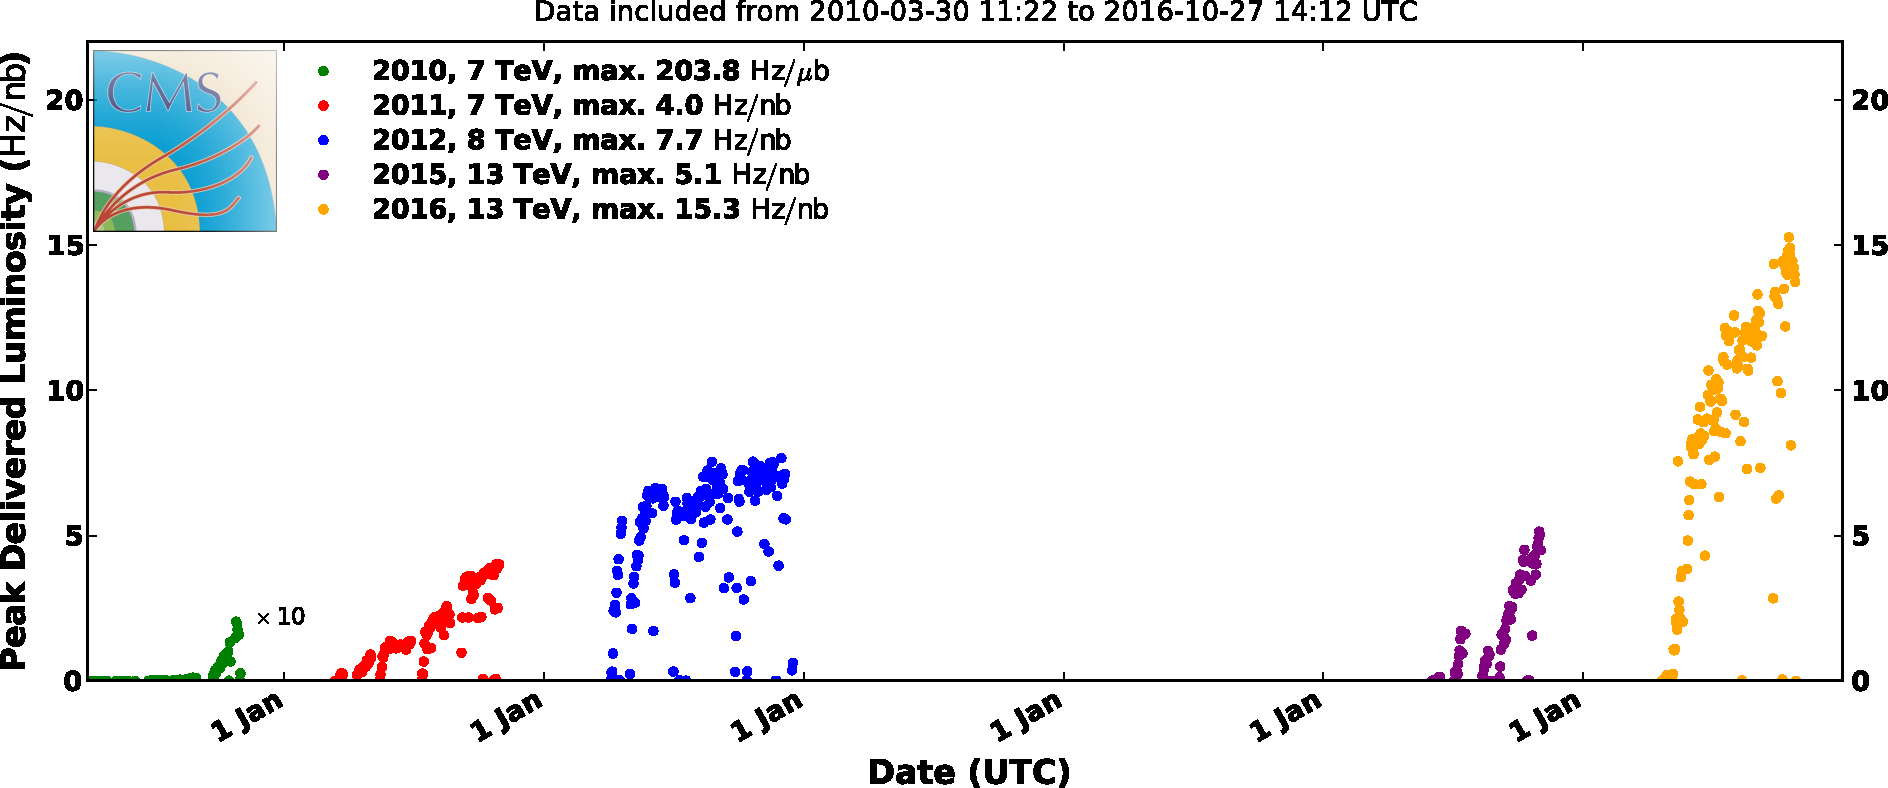
\includegraphics[width=0.95\textwidth]{figures/experiment/peak_lumi_pp.pdf}
}

During a bunch crossing multiple \acrlong{pp} interactions can occur which are referred to as \glshere{pu}. Their number on average is proportional to the luminosity times the total inelastic \gls{pp} cross section. In 2012, an average of 21~\acrlong{pu} interactions has been observed in 8~\TeV \gls{pp} collisions at the \gls{ip} of \gls{cms}. This increased in 2016 due to the higher luminosity and cross section at 13~\TeV to about 27~interactions on average.

\todo{can add a plot comparing all three pu profiles}

%##############################################
\subsection{Accelerator complex}
%##############################################

An overview of the accelerator complex at \gls{cern} is given in Fig.~\ref{fig:experiment-accelerator-complex} which includes the systems for filling the \gls{lhc} with bunches of protons or lead ions.

\myfigure{\label{fig:experiment-accelerator-complex}The accelerator complex at \gls{cern}. The figure is taken from Ref.~\cite{Mobs:2225847}.}{
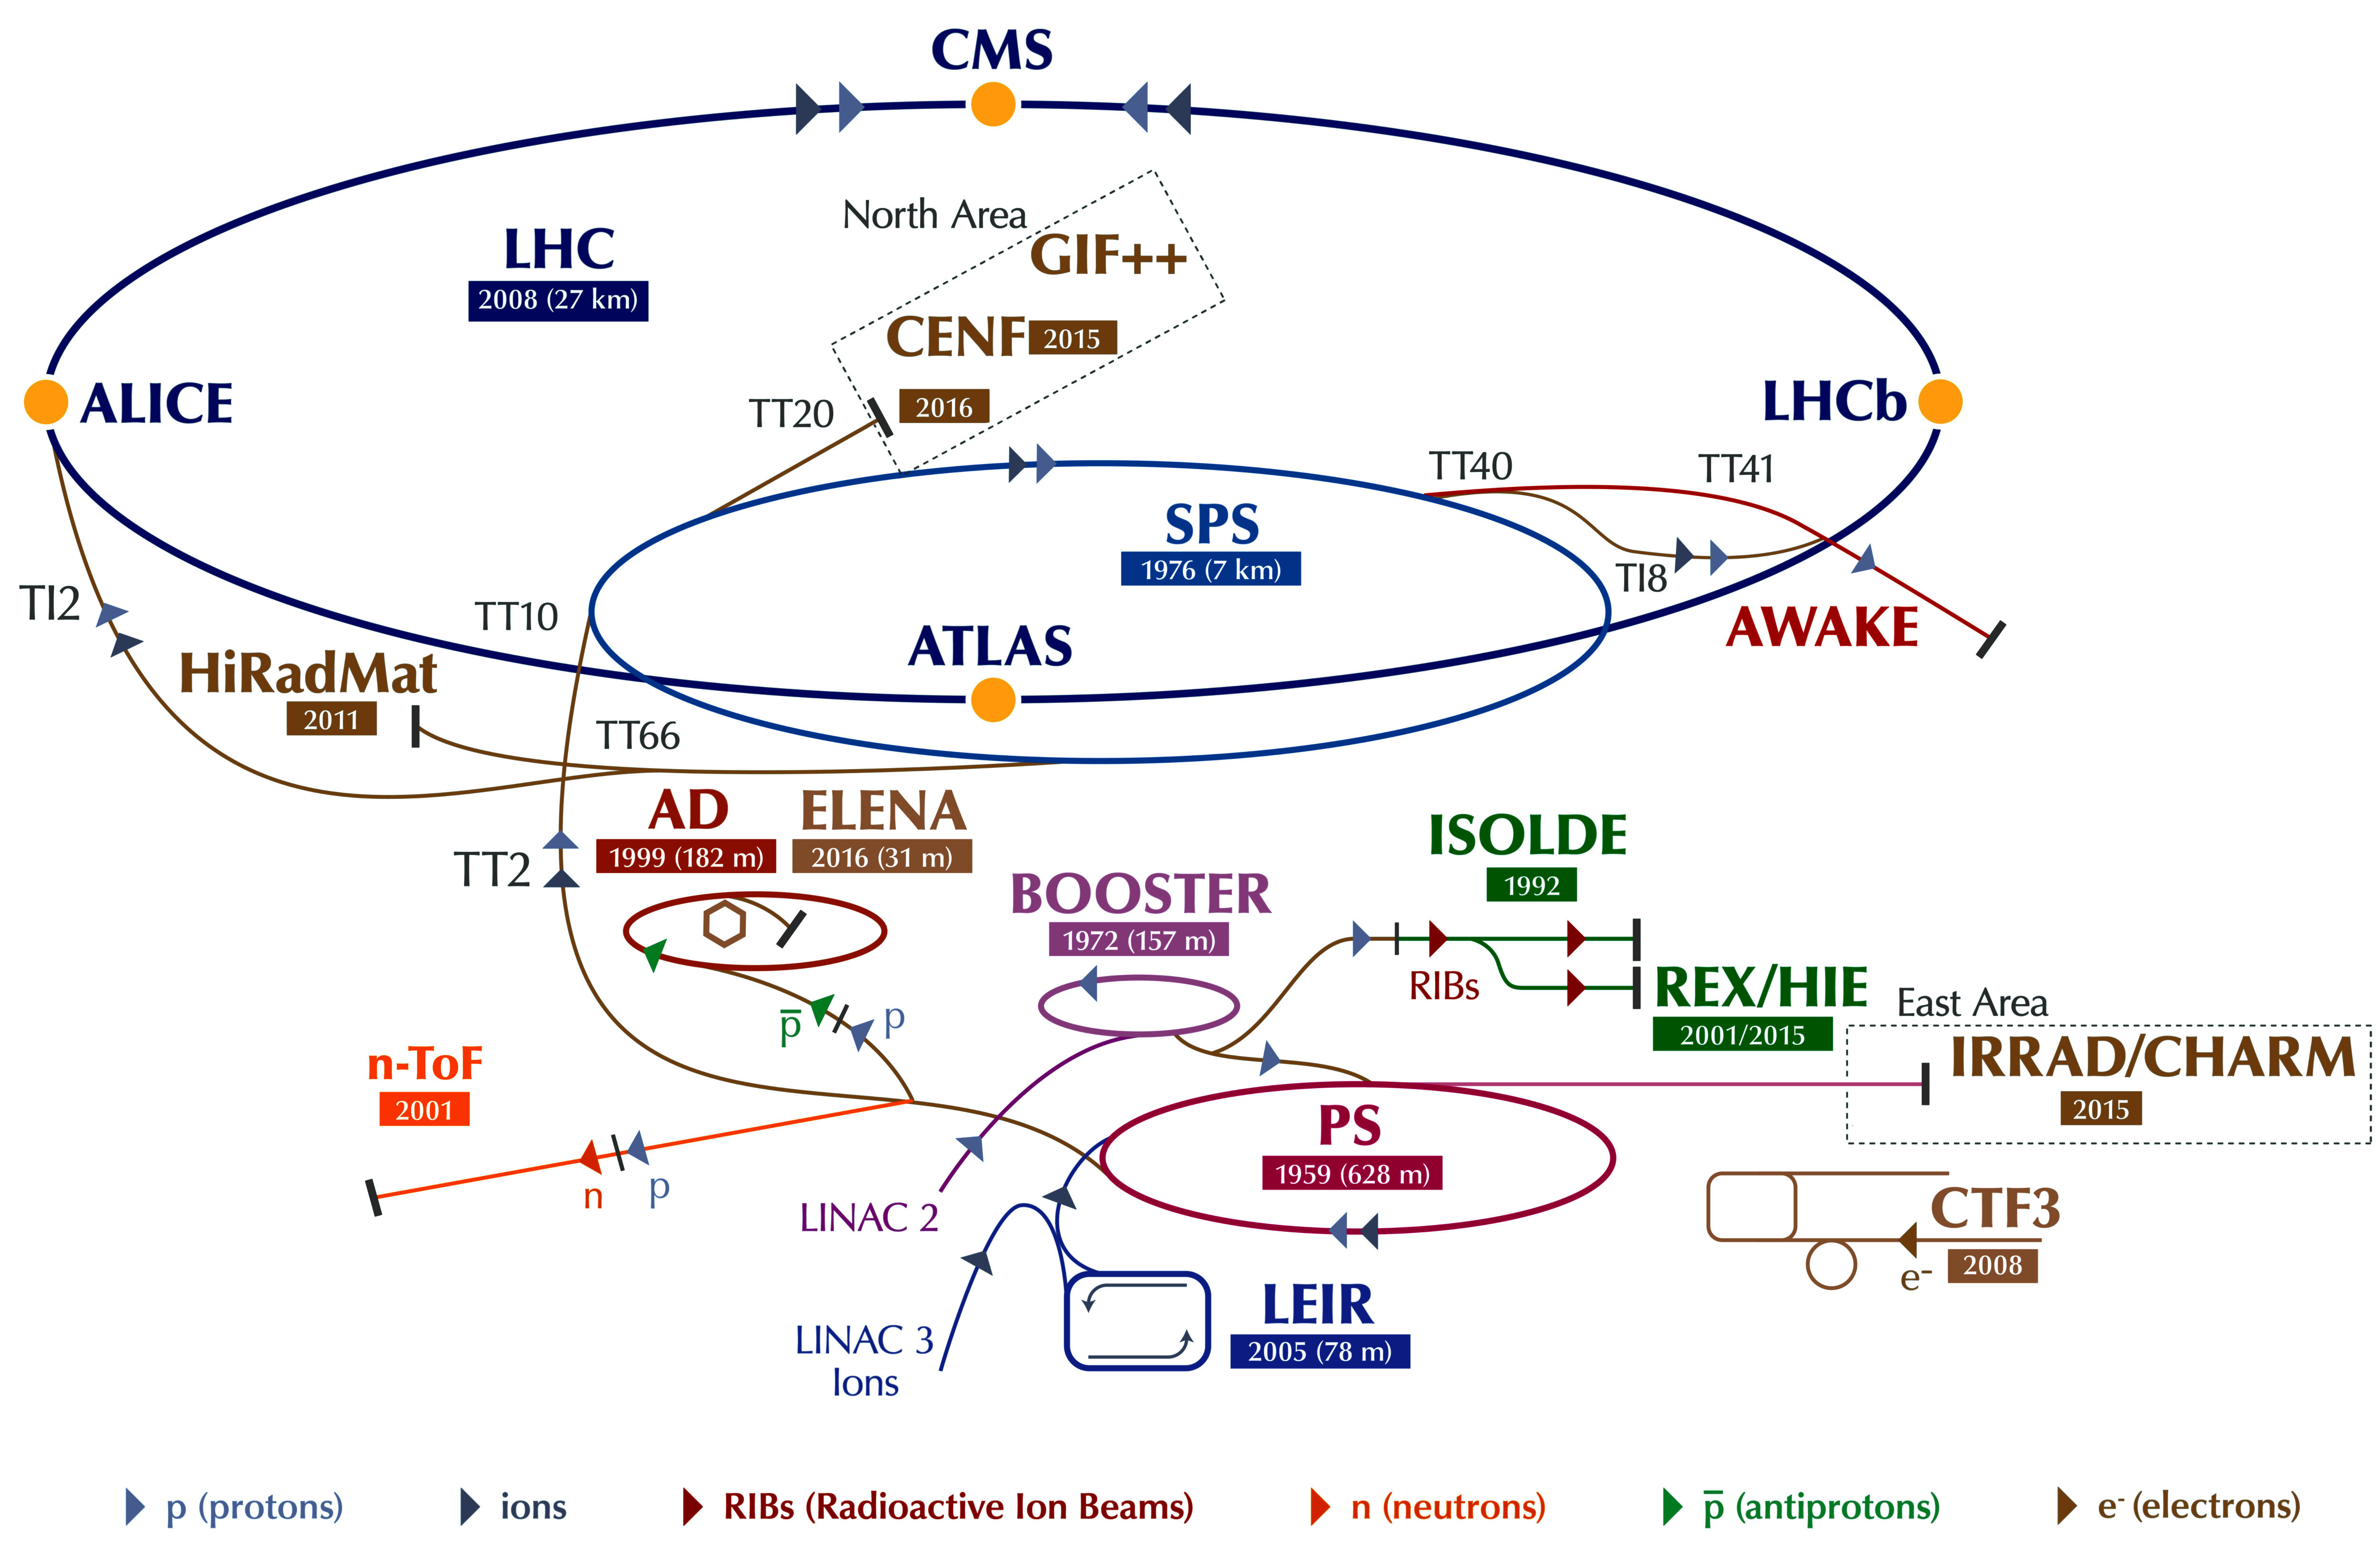
\includegraphics[width=0.99\textwidth]{figures/experiment/CERN_accelerator_complex.jpg}
}

The production sequence of proton bunches for the \gls{lhc} is as follows. In the linear accelerator ``Linac~2'' hydrogen atoms are stripped of their electron through an electric field. The remaining protons are accelerated to a momentum of 50~\MeV and injected into the \glshere{psb}. It consists of four vertically separated beam pipes which allow multi-turn injections to increase the bunch intensity which however also increases the transverse emittance~\cite{doi:10.1142/S0217751X13300196}. After accelerating the protons to 1.4~\GeV, the beams are injected into the \glshere{psync}. Here the required bunch spacing of 25~ns is formed. The standard procedure was to use only six bunches from two \gls{psb} cycles and split them first by three, accelerate them to 25~\GeV, and then split each again by two twice to produce in total 72~bunches with the required spacing~\cite{Benedikt:2001ar}. A new scheme called \glshere{bcms} was introduced in July, 2016. It utilizes all eight bunches from two \gls{psb} cycles which are first narrowed and then combined to four followed by the same splitting and acceleration procedure as before resulting in 48~bunches with a higher intensity and a lower transverse emittance~\cite{bcms}. After the \gls{psb} the proton bunches are injected into the \glshere{sps} and accelerated up to the \gls{lhc} injection energy of 450~GeV.


%##############################################
\subsection{Overview of experiments}
%##############################################

Various particle detectors are installed at the \gls{lhc} to record the outcome of proton-proton or heavy ion collisions. Four major detectors are directly located at the four \glspl{ip}. Two general purpose detectors are located at two high luminosity \glspl{ip}. These are the \glsmark{atlas}~\cite{Aad:2008zzm} and \glsmark{cms}~\cite{Chatrchyan:2008aa} experiments which have both a wide physics program ranging from precision measurements of the \glsunset{sm}\gls{sm} to searches for various kinds of new physics like extra dimensions, dark matter particles or \gls{susy}. Despite similar goals the technical realization of the two experiments is different. The \gls{atlas} detector is of cylindrical shape around the beam pipe with a length of 44~m and a diameter of 25~m. It consists of an inner tracking detector, a liquid argon electromagnetic calorimeter, a hadronic calorimeter, and a muon spectrometer with full $2\uppi$ coverage in the azimuthal angle. A detailed description of the \gls{cms} detector is given below in Sec.~\ref{sec:experiment-cms}. The two other major detectors are the \glsmark{alice}~\cite{Aamodt:2008zz} and \glsmark{lhcb}~\cite{Alves:2008zz} experiments which are more specialized. Their luminosity is intentionally leveled down by displacing the beams slightly at their \glspl{ip}~\cite{Follin:1955354}. The lower luminosity is required to reduce the number of pileup interactions and to prevent damage to the detectors through radiation. The \glsmark{alice} experiment focuses on heavy ion collisions in which the properties of quark-gluon plasma can be studied. The goals of the \glsmark{lhcb} experiment are precision measurements of \gls{cp}-violating processes and searches for rare decays of B~hadrons amongst others.

In addition, three smaller experiments, \glsmark{lhcf}~\cite{Adriani:2008zz}, \glsmark{totem}~\cite{Anelli:2008zza}, and \glsmark{moedal}~\cite{Pinfold:2009oia}, have been installed at the \gls{lhc} using certain fractions of the scattered particles from the \glspl{ip} of the \gls{atlas}, \gls{cms}, and \gls{lhcb} detectors, respectively. 


%##############################################
\section{CMS experiment}
%##############################################
\label{sec:experiment-cms}

The \glsmark{cms}~(Compact Muon Solenoid) experiment is a multipurpose particle detector whose goal is to record \gls{pp} and heavy ion collisions at high luminosities. It consists of a superconducting solenoid and multiple subdetectors as shown in Fig.~\ref{fig:experiment-cms} to track, reconstruct, and identify particles which traverse the detector each bunch crossing.

\myfigure{\label{fig:experiment-cms}Overview of the \gls{cms} subcomponents. The figure is taken from Ref.~\cite{Chatrchyan:2008aa}.}{
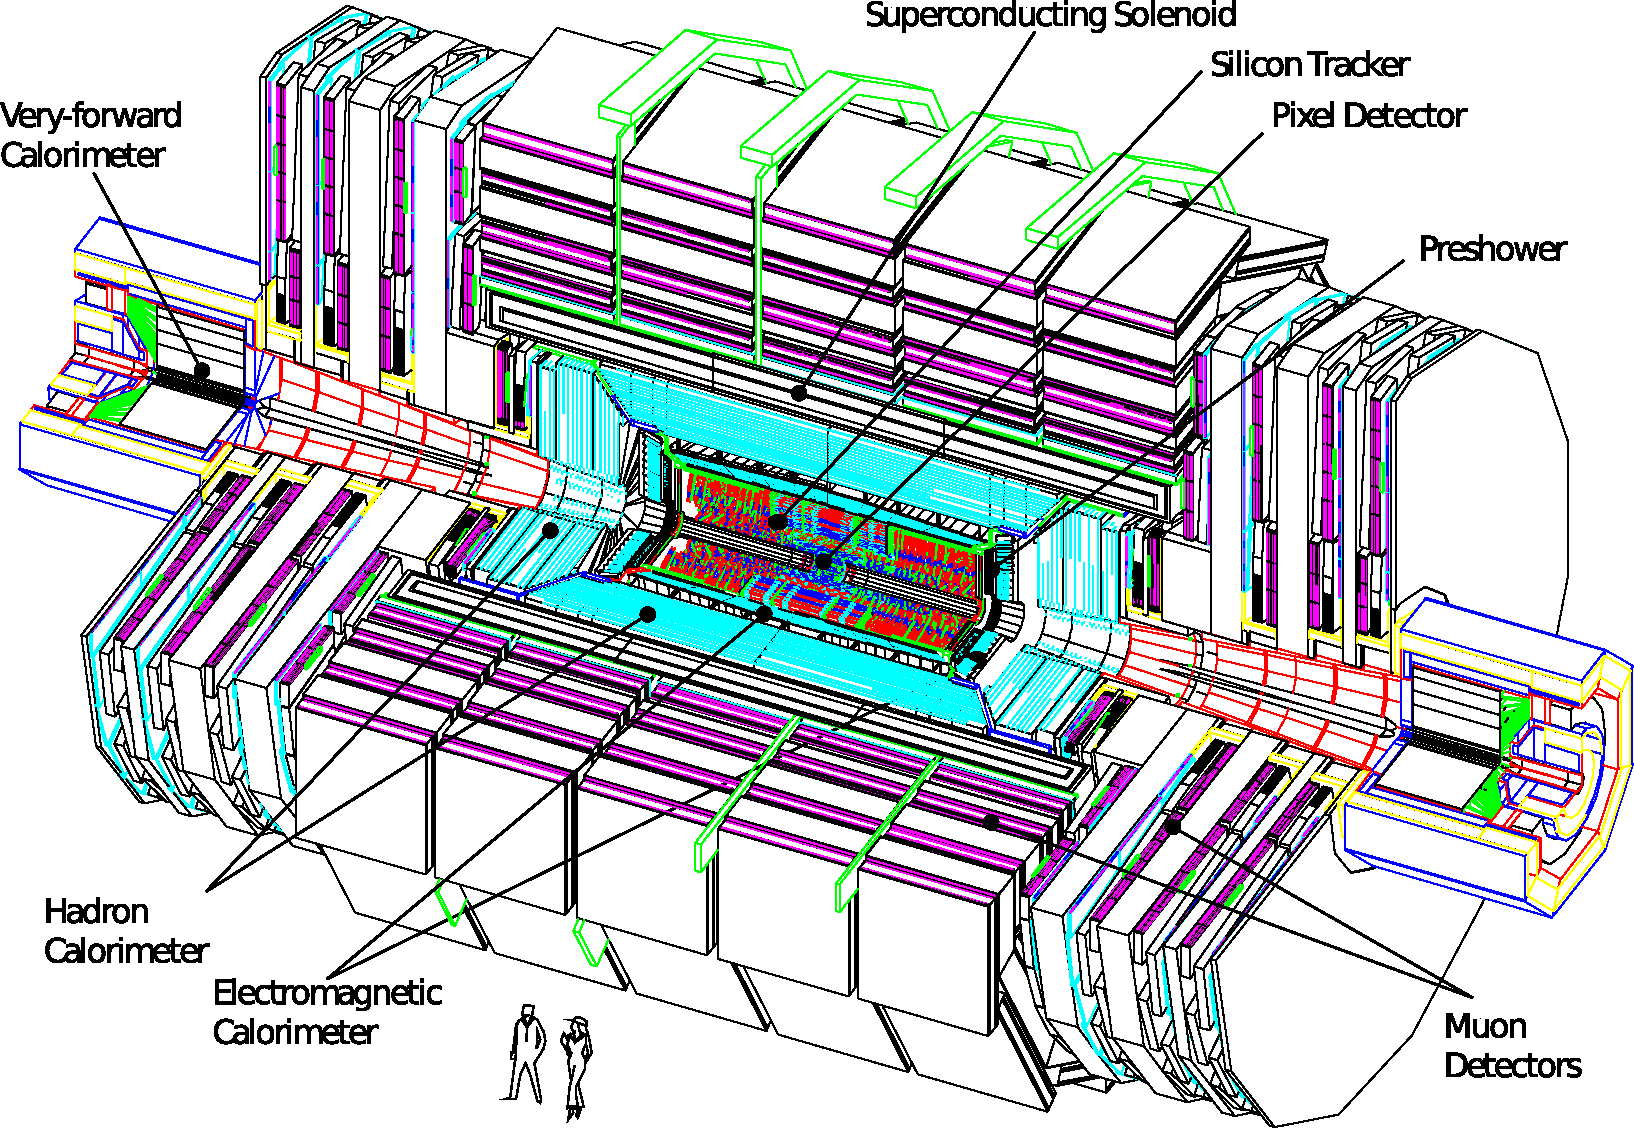
\includegraphics[width=0.99\textwidth]{figures/experiment/CMS_overview.pdf}
}

The detector is shaped cylindrically by layers in the barrel region and endcap disks in the forward regions around the beam pipe. It has an overall length of 21.6~m and a diameter of 14.6~m with a total weight of approximately 12\,500~tons. A right-handed coordinate system has been established whose center is located at the nominal \gls{ip}. It is oriented such that the y-axis points upwards, the x-axis points inwards to the center of the \gls{lhc} ring, and the z-axis points counterclockwise along the beam pipe. The azimuthal angle $\phi$ is defined in the transverse plane, spanned by the x- and y-axes, which lies perpendicular to the beam pipe. In this plane, the radius is defined as $r=\sqrt{x^2+y^2}$ which measures the distance to the z-axis. For a particle originating from the center with an energy $E$ and momentum $p_\mathrm{z}$ along the z-axis one defines its rapidity as

\begin{equation}
y=\frac{1}{2}\ln\left(\frac{E+p_\mathrm{z}}{E-p_\mathrm{z}}\right)\,. \label{eq:experiment-rapidity}
\end{equation}

The advantage of the rapidity over the usage of the angle $\theta$ measured from the z-axis is that differences of rapidities are invariant under Lorentz-boosts. Furthermore, in the case of a massless particle, the rapidity is equal to the pseudorapidity

\begin{equation}
\eta=\mathrm{artanh}\left(\frac{p_\mathrm{z}}{|\vec{p}|}\right)=-\ln\left[\tan\left(\frac{\theta}{2}\right)\right]\,. \label{eq:experiment-pseudorapidity}
\end{equation}

In the following, the components of \gls{cms} are briefly described and their purpose is motivated. Further information can be found in Refs.~\cite{Chatrchyan:2008aa,Bayatian:922757}.


%##############################################
\subsection{Solenoid magnet}
%##############################################

The solenoid magnet is a central part of the \gls{cms} detector. It enables momentum measurements of charged particles by analyzing their curved trajectories with the inner tracking system. Additionally, the muon system located in the outer return flux of the magnetic field allows to measure the momenta of muons originating from the \gls{ip} a second time. The design of \gls{cms} was particularly motivated to achieve a good resolution of muon momenta and dimuon mass spectra which are key ingredients when searching for new resonances like the at that time undiscovered Higgs boson~\cite{Acquistapace:1997fm}.

The magnet consists of four layers of superconducting \gls{nbti} cables. It is placed in a cold mass within a vacuum tank which is cooled down to 4.7~K using liquid helium. To guide the return flux of the magnetic field, a large iron yoke has been installed. It consists of five 12-sided barrel wheels in three layers with a length of 11~m and six endcap disks. In design the solenoid is capable of producing a homogeneous magnetic field of up to 4~T in its inner free bore which has a diameter of 6~m and a length of 12.5~m. However, the magnet has been operated with a reduced current of 18164~A so far yielding a slightly lower field of 3.8~T~\cite{Chatrchyan:2009si}. 



%##############################################
\subsection{Inner tracking system}
%##############################################
\label{sec:experiment-tracker}

The inner tracking system is located closest to the beam pipe and has a total length of 5.8~m with a diameter of 2.5~m. It is used to find trajectories of charged particles which are bent by the magnetic field. Their momentum, charge, and point of origin is estimated in the track reconstruction.

At design luminosity approximately 1\,000 particles traverse the tracking system per bunch crossing on average. This yields a hit rate density of about $1~\mathrm{MHz/mm^2}$ at an inner radius of 4~cm which is reduces to $3~\mathrm{kHz/mm^2}$ at the outer edge of the tracker. The tracker modules are based on doped silicon semiconductors which are operated in reverse mode to detect the traversing of charged particles through ionization. This technology allows for modules with a sufficiently high granularity and a fast response time that are also able to operate in such high radiation environments.

The system consists of various parts with different module types as shown in Fig~\ref{fig:experiment-tracker}. In total it covers a pseudorapidity range of $|\eta|<2.5$. Pixel modules are located next to the beam pipe where the particle flux is particularly high. They are installed in three barrel layers~(\glsmark{bpx}) at radii of 4.4, 7.3, and 10.3~cm, and in two endcap disks~(\glsmark{fpx}) per side. A pixel module has a cell size of $100\times150~\upmu\mathrm{m}^{2}$ which allows a two-dimensional local hit position measurements. Local positions are transformed into three-dimensional global positions by accounting for the surface orientation of each module. The channel occupancy of the pixel subdetector, which is defined as the fraction of active readout channels, has been measured in data and ranges between 0.002\range0.02\% only~\cite{Chatrchyan:2014fea}. This facilitates the search for particles trajectories in recorded hit patterns by starting from the precise hits on the pixel modules.

\myfigure{\label{fig:experiment-tracker}Overview of the \gls{cms} tracking system. The figure is taken from Ref.~\cite{Chatrchyan:2014fea}.}{
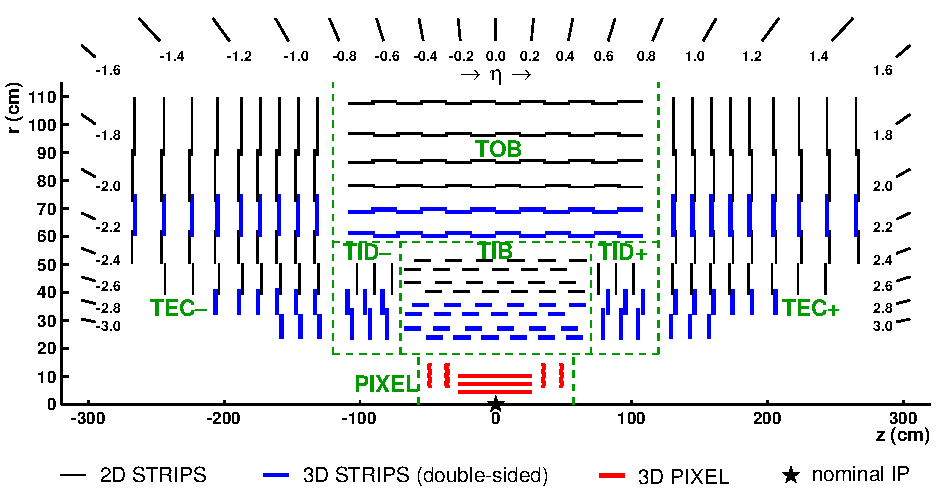
\includegraphics[width=0.99\textwidth]{figures/experiment/CMS_tracker.pdf}
}

Silicon strip modules are installed in the other parts of the inner tracking system. They are organized in four inner barrel layers~(\glsmark{tib}) at radii of 20\range50~cm; six outer barrel layers~(\glsmark{tob}) at radii of 55\range116~cm; three inner endcap disks~(\glsmark{tid}); and nine outer endcap disks~(\glsmark{tec}). In the barrel, the strip directions on each module are aligned along the z-axis with a strip-to-strip distance that varies between $80\range183~\upmu\mathrm{m}$. In the endcap disks, the modules are wedge-shaped with their strips running along the radial axis whose distance ranges between $100\range184~\upmu\mathrm{m}$. They are cooled down and operated below $-10^\circ\mathrm{C}$ to counteract the heat produced by the electronics and to improve their lifetime. The strips allow to measure a local one-dimensional hit position perpendicular to their direction. However, a few layers and disks contain double-sided strip modules as indicated in Fig.~\ref{fig:experiment-tracker} which are tilted by an angle of 0.1~rad with respect to each other. Those modules allow to reconstruct 2D hits by matching two 1D hits from both sides together. 


%##############################################
\subsection{Electromagnetic calorimeter}
%##############################################

The electromagnetic calorimeter~(\glsmark{ecal}) encloses the inner tracker and covers a pseudorapidity range of $|\eta|<3$. It consists of scintillating lead tungstate~($\mathrm{PbWO}_{4}$) crystals to detect electromagnetic showers originating from charged or neutral particles (especially photons and electrons) in the crystals. In particular, the capability of detecting a diphoton resonance from Higgs boson decays has been one of its design goals.

An overview of the \gls{ecal} layout is displayed in Fig.~\ref{fig:experiment-ecal}. In total 61\,200 crystals in the shape of a truncated pyramid are installed in the barrel and 7\,324 in each of the two endcaps. The barrel crystals have a length of 23~cm and a rectangular front cross section of $22\times22~\mathrm{mm}^{2}$. In the endcaps the crystals have a similar shape with a length of 22~cm and a front cross section of $28.62\times28.62~\mathrm{mm}^{2}$. The crystals are slightly tilted such that no particle originating from the nominal \gls{ip} can pass the \gls{ecal} through a crack between the crystals within its acceptance.

\myfigure{\label{fig:experiment-ecal}Overview of the \gls{cms} electromagnetic calorimeter system. The figure is taken from Ref.~\cite{Bayatian:922757}.}{
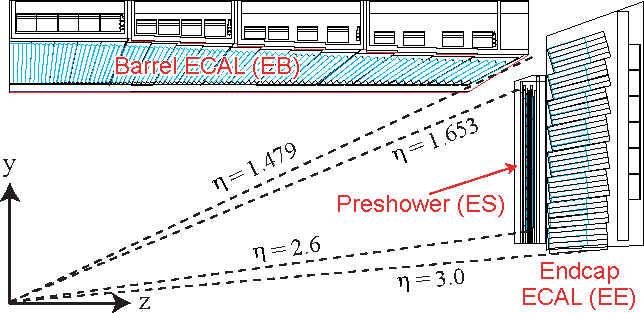
\includegraphics[width=0.75\textwidth]{figures/experiment/CMS_ecal.pdf}
}

The crystal material was chosen for its high density of $8.28~\mathrm{g}/\mathrm{cm}^{3}$, short radiation length of 0.89~cm, and radiation hardness. In addition, the spatial extension of an electromagnetic shower inside the crystals, the so-called Moli\`ere radius, amounts to only 2.2~cm which yields a good position resolution and shower separation. The crystals emit about 4.5 photoelectrons per \MeV with a wavelength of 420\range430~nm. About 80\% of the light is emitted within 25~ns after an electromagnetic shower occurred. In the barrel the signal of the collected photons is amplified by \glsplhere{apd} whereas in the endcaps \glsplhere{vpt} are used instead which are specifically designed to operate also in the axial magnetic field. The energy resolution of the crystals has been measured in electron beams for energies $20<E<250~\GeV$~\cite{Adzic:2007mi}. It can be parameterized as

\begin{equation}
\left(\frac{\sigma}{E}\right)^{2}=\underbrace{\left(\frac{2.8\%}{\sqrt{E/\GeV}}\right)^{2}}_\text{stochastic}+\underbrace{\left(\frac{0.12}{E/\GeV}\right)^{2}}_\text{noise}+\underbrace{\big(0.30\big)^{2}}_\text{constant}
\end{equation}

which yields for example a resolution of $0.43~\GeV$ at an electron energy of $100~\GeV$.

In front of the two \gls{ecal} endcaps the preshower detector~(\glsmark{es}) is located which covers a pseudo rapidity range of $1.652<|\eta|<2.6$. It consists of two layers of lead radiators to initiate electromagnetic showers with a layer of silicon strip sensors after each radiator for measuring the transverse profile of a shower. This allows to identify neutral pions and improves the identification and position measurement of electrons and photons.


%##############################################
\subsection{Hadron calorimeter}
%##############################################

The hadron calorimeter~(\glsmark{hcal}) is a sampling calorimeter and organized in four parts as shown in Fig.~\ref{fig:experiment-hcal}. It covers a pseudorapidity range of $|\eta|<5$ in total. Its function is to initiate and detect hadronic showers from particles such as protons, neutrons, kaons, and pions which allows to measure their position and energy. Furthermore, it helps to determine the transverse momentum imbalance of an event since the only remaining particles from a collision that are not stopped by the \gls{hcal} are neutrinos and muons where the latter are however identified and measured in the muon system as discussed later in Sec.~\ref{sec:experiment-muon-systems}.

\myfigure{\label{fig:experiment-hcal}Overview of the \gls{cms} hadronic calorimeter system. The figure is taken from Ref.~\cite{Chatrchyan:2008aa}.}{
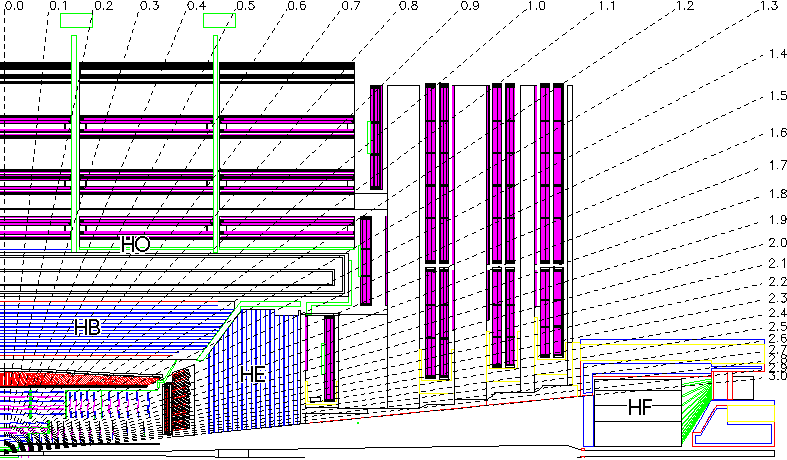
\includegraphics[width=0.95\textwidth]{figures/experiment/CMS_hcal.pdf}
}

The central hadron calorimeter, consisting of a barrel~(\glsmark{hb}) and two endcap~(\glsmark{he}) regions, is located directly after the \gls{ecal} and extends up to the solenoid. The \gls{hb} covers a pseudorapidity range of $|\eta|<1.3$. It consists of brass absorber plates in 14~layers oriented along the z-axis with a thickness of 50.5~mm~(first eight) and 56.5~mm~(last six), respectively. For structural support two additional layers of 40~mm and 50.5~mm thick steel absorber plates are installed at its inner and outer rim respectively. Between the absorbers 72~azimuthal wedges of plastic scintillators in 17~layers with a thickness of 3.7~mm or 9~mm are installed where each covers a segment of $\Delta\eta\times\Delta\phi=0.087\times0.087$. Their emitted light is optically added per tower and guided through \glshere{wls} fibers to \glsplhere{hpd} located at the end of the \gls{hb} structure. The \gls{hb} has a depth of 5.8 interaction lengths at $\eta=0$ which increases with pseudorapidity and amounts to 10.4 interaction lengths at $|\eta|=1.3$. 

The same design of alternating brass absorbers~(79~mm thick) with 17~scintillator layers in between and \gls{wls} fibers for readout is utilized in the \gls{he}. It covers a pseudorapidity range of $1.3<|\eta|<3$ and has a depths of about 10~interaction lengths. Its granularity increases from $\Delta\eta\times\Delta\phi=0.087\times0.087$ to $0.17\times0.17$ for $|\eta|>1.6$.

To contain hadronic showers in the barrel region further, an additional calorimeter, the hadron outer calorimeter~(\glsmark{ho}), is placed directly at the outside of the solenoid utilizing it as absorber. It consists of one or two layers of scintillators, depending on the pseudorapidity, which match the granularity of the \gls{hb}. This extends the depths of the combined \gls{hb}+\gls{he}+\gls{ho} system to an overall minimum of 11.8 interaction length with the exception of the \gls{hb}-\gls{he} transition region~($|\eta|\sim 1.3$).

An additional calorimeter system, the hadron forward calorimeter~(\glsmark{hf}), is located 11.2~m away from the \gls{ip} at both sides where it covers a pseudorapidity range of $3<|\eta|<5.2$. The \gls{hf} is of particular importance for this thesis since the signature of $t$-channel single-top-quark events features a characteristic forward jet that is often detected within its acceptance. For the \gls{hf} a different detector technology was chosen to withstand the expected higher levels of radiation of about $1~\mathrm{MGy/a}$ occurring in the forward region. It uses quartz fibers to detect Cherenkov light from the electromagnetic component of a shower. The fibers are oriented along the z-axis and placed in grooves within steel plates which act as absorbers. The fibers are arranged to achieve a granularity of $\Delta\eta\times\Delta\phi=0.175\times0.175$. Only half of the fibers extend over the complete \gls{hf} depth of 165~cm which corresponds to 10 interaction lengths. The other half starts at a depth of 22~cm instead. Since electromagnetic showers are typically shorter than hadronic ones the two shower types can be disentangled from each other by comparing the separated readouts from the long and short fibers. The produced Cherenkov light is guided to \glsplhere{pmt} located behind a shield of 40~cm steel and polyethylene slabs which protects them from the high radiation.

The energy response of the \gls{hcal} modules has been measured in pion beams with energies of $20<E<300~\GeV$~\cite{Baiatian:1049915}. This results in 

\begin{equation}
\left(\frac{\sigma_\mathrm{\gls{hb}+\gls{he}}}{E}\right)^{2}=\left(\frac{115\%}{\sqrt{E/\GeV}}\right)^{2}+\big(5.5\%\big)^{2}
\end{equation}

for the combined \gls{hb}+\gls{he} system which is found in agreement with simulation. For the \gls{hf} resolutions of

\begin{equation}
\left(\frac{\sigma_\mathrm{\gls{hf}}}{E_\mathrm{e}}\right)^{2}=\left(\frac{198\%}{\sqrt{E/\GeV}}\right)^{2}+\big(9\%\big)^{2}\,,\quad \left(\frac{\sigma_\mathrm{\gls{hf}}}{E_{\uppi}}\right)^{2}=\left(\frac{280\%}{\sqrt{E/\GeV}}\right)^{2}+\big(11\%\big)^{2}
\end{equation}

have been measured in electron and pion test beams respectively~\cite{Bayatian:2006jz}.



%##############################################
\subsection{Muon system}
%##############################################
\label{sec:experiment-muon-systems}

A major design goal of \gls{cms} is the precise and robust detection of muons to achieve a good dimuon mass resolution~($1\%$ at $100~\GeV$) and charge determination over a wide muon momentum range of up to 1~\TeV and beyond. Muons are a key ingredient to detect signatures of various \gls{sm} processes and beyond as for example in Higgs bosons studies where their decay to four muons via intermediate Z~bosons is analyzed. In particular, events containing a single muon amongst others that may stem from the decay of a single top quark are analyzed in this thesis.

The muon system is located at the outside of the \gls{cms} detector within the gaps of the iron yoke. It consists of three types of gaseous detectors. Muons passing through the gas will ionize it. A strong electric field pulls the freed electrons then to wires and the resulting electric pulse is read out. The choice of the gas mixture together with the electric field strength lets the drifting electrons ionize the gas further close to the wire which amplifies the pulse. An overview of the muon system is provided in Fig.~\ref{fig:experiment-muons}. \Glsplhere{dt} are installed in the barrel~($|\eta|<1.2$) where the muon flux is relatively low. In the endcaps~($0.9<|\eta|<2.4$) \glsplhere{csc} are used which can operate in the higher muon flux environment and in the inhomogeneous magnetic field. In addition, \glsplhere{rpc} are installed in the barrel and endcaps as a complementary system with a coverage of $|\eta|<1.6$.

\myfigure{\label{fig:experiment-muons}Overview of the \gls{cms} muon system by the end of \gls{lhc} \gls{run1}. The figure is taken from Ref.~\cite{Chatrchyan:2013sba}.}{
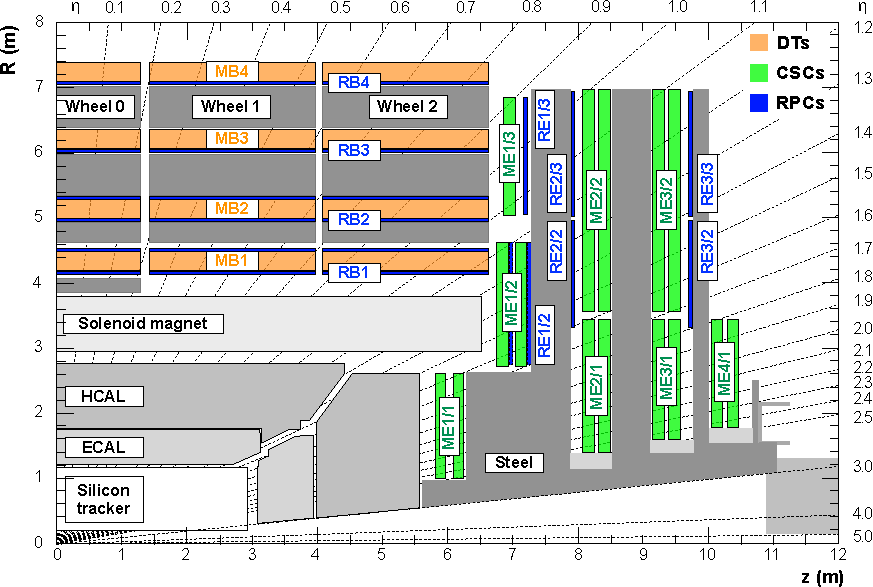
\includegraphics[width=0.85\textwidth]{figures/experiment/CMS_muons.pdf}
}

The \glspl{dt} consist of nearly rectangular cells with a cross section of $42\times 13~\mathrm{mm}^{2}$ in which a $50~\upmu\mathrm{m}$ thick and 2.4~m long gold-plated steel wire is spanned through the center. The cells are filled with a gas mixture of 85\%~Ar and 15\%~$\mathrm{CO}_{2}$ which yields an amplification of $10^{5}$ and a drift time of about 380~ns for a maximum drift length of 21~mm. The \glspl{dt} are organized in four layers which form an independent gas-tight super layer unit. A \gls{dt} chamber consists of three (or two) super layers where the wires in the first and last layers are oriented along the z-axis and the wires in the middle layer are oriented orthogonal along the $\phi$ direction. Four layers of \glspl{dt} chambers are placed in the barrel region with 60~chambers in each of the inner three layers and 70 in the outer one which amounts to about 172\,000 wires in total.

In the endcaps trapezoidal-shaped \glspl{csc} are installed in four disks per side. Each disk consists of 18~or 36~chambers which are slightly overlapping to ensure full azimuthal coverage. The \glspl{csc} are multiwire proportional chambers where each consists of seven radially-oriented cathode strips glued on 12.7~mm-thick panels. Their pitch changes radially from 8.4~mm to 16~mm at the outside. Six azimuthally-oriented wires are placed in the gas gaps between the panels with a width of 9.5~mm. A gas mixture of 40\%~Ar, 50\%~$\mathrm{CO_{2}}$, and 10\%~$\mathrm{CF}_{4}$ is used which yields a gain of about $7\times10^{4}$ at a voltage of $3.6~\mathrm{kV}$. Since the first inner \glspl{csc}~(labeled ME1/1) are located inside the solenoid a slightly different design with tilted wires by $29^{\circ}$ was chosen to compensate for the Lorentz drift in the magnetic field. The fourth \gls{csc} disk labeled ME4/2 (not present in Fig.~\ref{fig:experiment-muons}) has been installed after \gls{run1} which adds an additional redundancy for muons within $1.2<|\eta|<1.8$~\cite{Wulsin:2015shd}.

The muon system is completed by \glspl{rpc} in the barrel and endcaps. These are gaseous parallel-plate detectors with two gaps of 2~mm width each. They provide a much shorter time resolution than the \glspl{dt} and \glspl{csc} of about 1~ns. Hence, they are used to associate a muon signal to the corresponding \gls{lhc} bunch crossing. In the barrel six layers of \glspl{rpc} are installed with their strips oriented along the z-axis. Their pitch varies per layer such that an azimuthal granularity of $5/16^\circ$ is achieved. In the endcaps four \gls{rpc} disks are installed with radially oriented strips. A fourth endcap disk was added after \gls{run1} as well~\cite{Tytgat:2012xi}.



%##############################################
\subsection{Data acquisition}
%##############################################


The \gls{cms} trigger and data acquisition system~\cite{Cittolin:578006,Bawej:2015tmz} deals with the individual readouts of the various subdetector front-end systems. It associates them to an event and finally transmits a file of multiple events to the \gls{cern} computing cluster for storage. A two-staged event triggering system is employed whose aim is to reduce the high data rate and to select only events for storage of certain physics interest. The event rate from the bunch crossing frequency of 40~MHz is reduced to about 100~kHz after the first stage, the \glshere{l1} trigger, and then to less than 1~kHz after the final \glshere{hlt} system.

The data acquisition starts at the subdetector systems where the individual channel readouts are stored continuously in pipelined buffers at a rate of 40~MHz. The \gls{l1} trigger system analyzes only the readout of the calorimeter and muon systems per bunch crossing to reach a decision within a maximum latency of $3.2~\upmu\mathrm{s}$. It consists of \glsplhere{fpga} which enable a flexible adaptation of the system to potential varying conditions and needs. The regional~(\glsmark{rct}) and global calorimeter trigger systems~(\glsmark{gct}) attempt to locate electron, photon, jet, and $\tau$-jet candidates from coarsely segmented \gls{ecal} and \gls{hcal} readouts. Additional pieces of information like the missing transverse energy and number of jets are also determined. The global muon trigger system~(\glsmark{gmt}) attempts to find muon candidates by using local information from the independent \gls{dt}, \gls{csc}, and \gls{rpc} trigger systems. In addition, a muon is considered isolated if the hadronic activity in its vicinity (provided by the \gls{gct}) is below a certain threshold. The final \gls{l1} decision is taken by the \glshere{gt} based on the candidates found by the \gls{gct} and \gls{gmt} systems.

After a positive \gls{l1} decision is received the individual readout fragments with a size of up to 8~kB are transfered via optical links to readout units~(\glsplmark{ru}) by \glsplhere{fed} where multiple fragments are merged. Event builder units~(\glsplmark{bu}) pick up the fragments via a high speed, Infiniband-based switching network from the \glspl{ru} and assemble the events.
The \gls{hlt} system then reads the assembled events from the \glspl{bu} via an Ethernet network. Its triggering rules are part of the standard \gls{cms} software~(\glsmark{cmssw}~\cite{Bayatian:922757}) which is invoked on a special computing farm called filter units~(\glsplmark{fu}). Starting from \gls{l1} candidates, the complete readout of an event is subjected to a sequence of reconstruction and filtering steps to reach a \gls{hlt} decision. One output file is created per \gls{cmssw} process, \gls{hlt} stream, and luminosity section where the latter corresponds to a period of about 23~s. Streams and files of selected events are merged in two steps on the \glspl{fu} and \glspl{bu} before they are transfered to the \gls{cern} computing center for full reconstruction.
